\documentclass{standalone}
\usepackage{tikz}
\usetikzlibrary{patterns, positioning}
\usepackage[sfdefault]{ClearSans} %% option 'sfdefault' activates Clear Sans as the default text font
\usepackage[T1]{fontenc}

\begin{document}
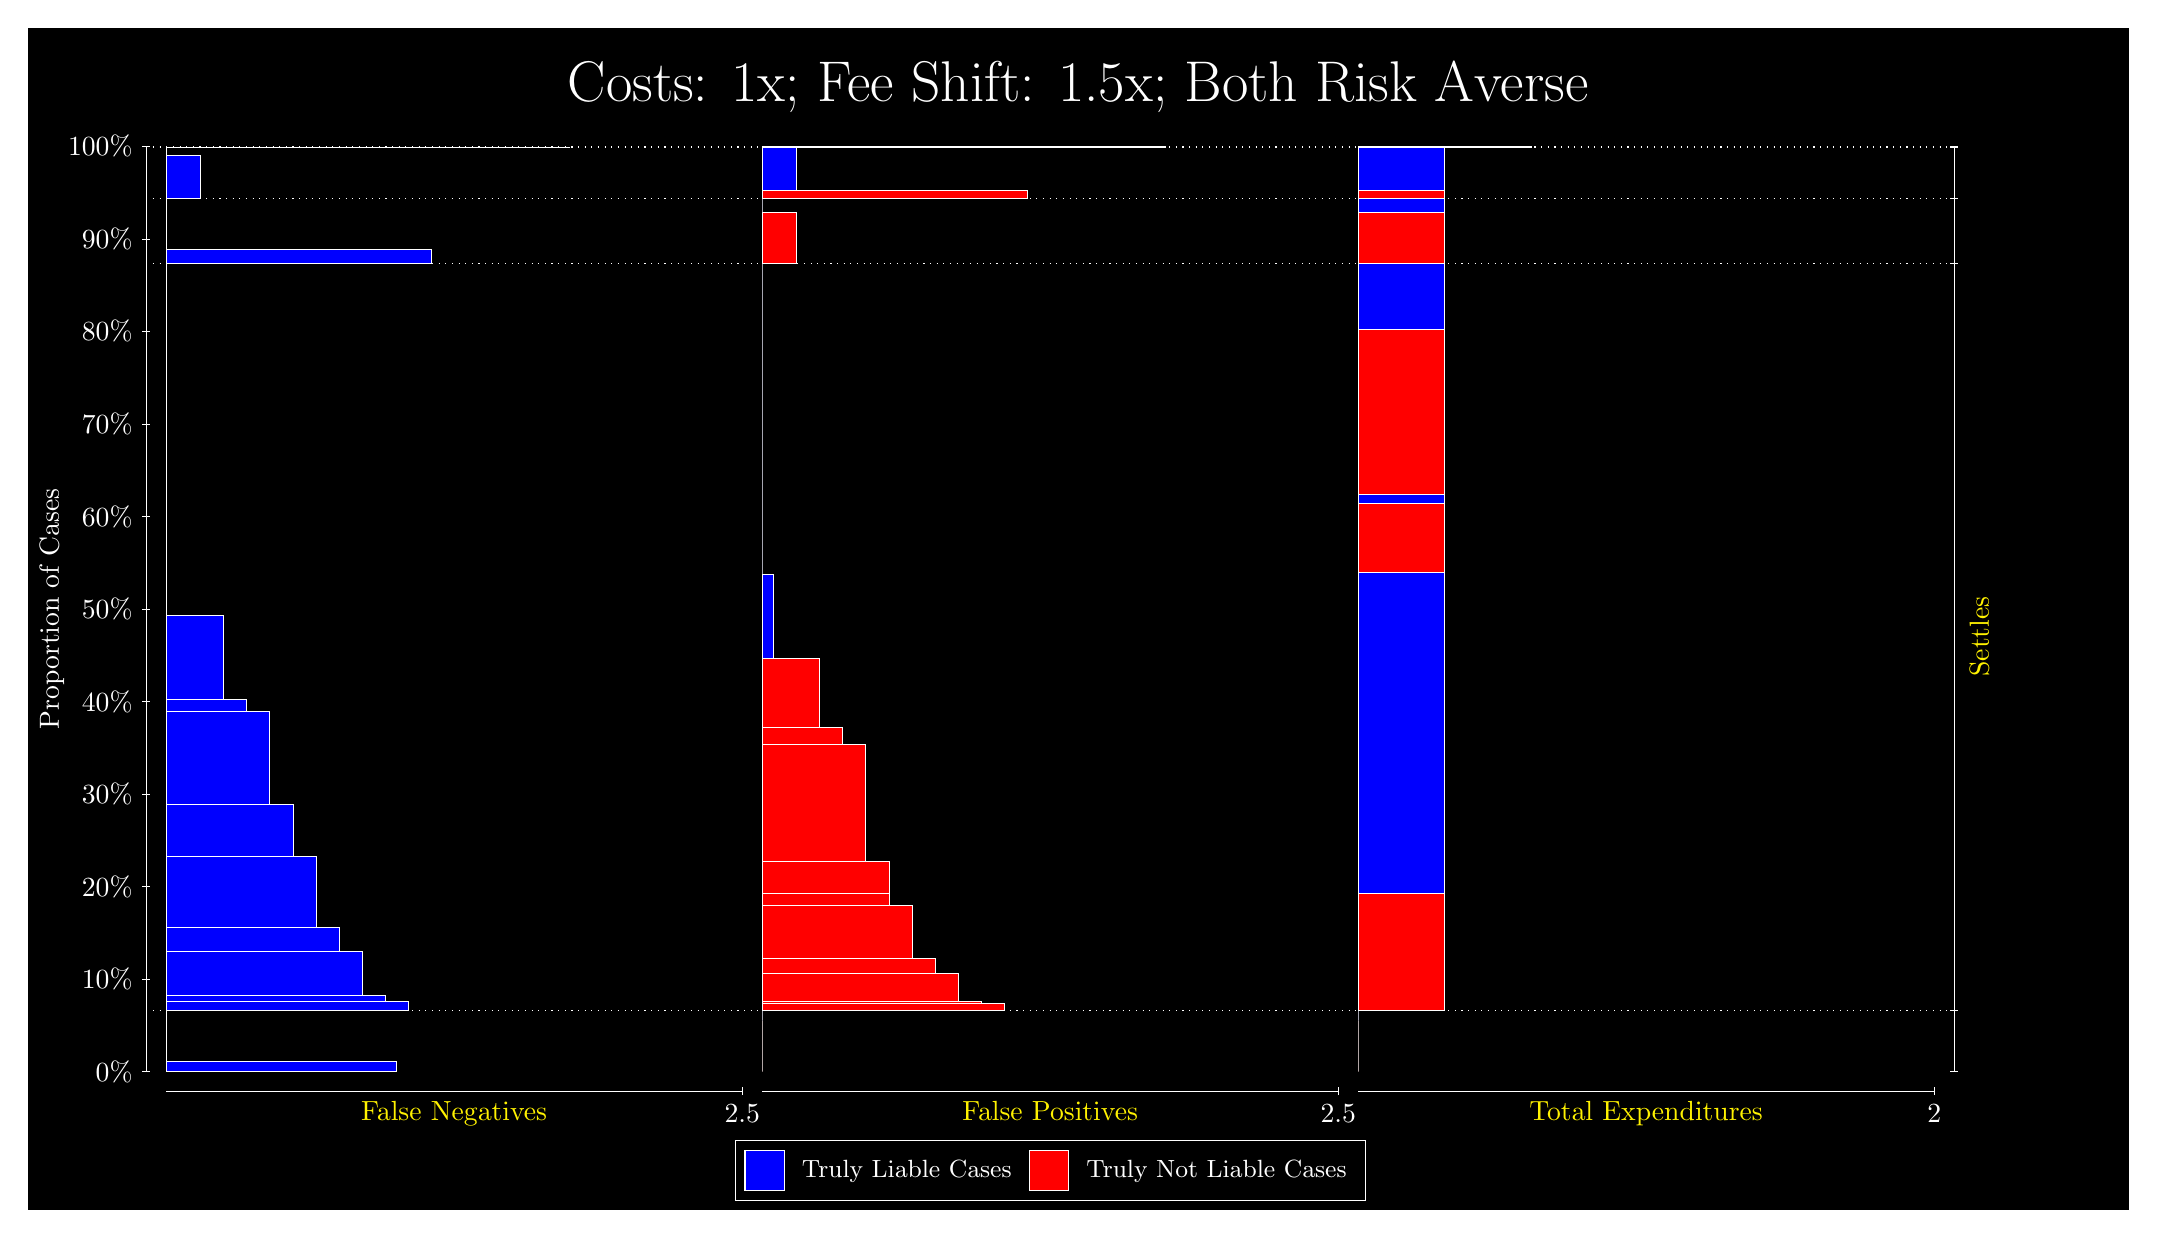
\begin{tikzpicture}
\draw[fill=black] (0,0) rectangle (26.667,15);
\draw[text=white] (0,13.5) rectangle (26.667,15) node[midway] {\huge Costs: 1x; Fee Shift: 1.5x; Both Risk Averse};
\draw[white, very thin] (1.5,1.75) -- (1.5,13.5);
\node[rotate=90, text=white, anchor=center] at (0.3, 7.625) {Proportion of Cases};
\draw[white, very thin] (1.45,1.75) -- (1.55,1.75);
\node[text=white, anchor=east] at (1.45, 1.75) {0\%};
\draw[white, very thin] (1.45,2.925) -- (1.55,2.925);
\node[text=white, anchor=east] at (1.45, 2.925) {10\%};
\draw[white, very thin] (1.45,4.1) -- (1.55,4.1);
\node[text=white, anchor=east] at (1.45, 4.1) {20\%};
\draw[white, very thin] (1.45,5.275) -- (1.55,5.275);
\node[text=white, anchor=east] at (1.45, 5.275) {30\%};
\draw[white, very thin] (1.45,6.45) -- (1.55,6.45);
\node[text=white, anchor=east] at (1.45, 6.45) {40\%};
\draw[white, very thin] (1.45,7.625) -- (1.55,7.625);
\node[text=white, anchor=east] at (1.45, 7.625) {50\%};
\draw[white, very thin] (1.45,8.8) -- (1.55,8.8);
\node[text=white, anchor=east] at (1.45, 8.8) {60\%};
\draw[white, very thin] (1.45,9.975) -- (1.55,9.975);
\node[text=white, anchor=east] at (1.45, 9.975) {70\%};
\draw[white, very thin] (1.45,11.15) -- (1.55,11.15);
\node[text=white, anchor=east] at (1.45, 11.15) {80\%};
\draw[white, very thin] (1.45,12.325) -- (1.55,12.325);
\node[text=white, anchor=east] at (1.45, 12.325) {90\%};
\draw[white, very thin] (1.45,13.5) -- (1.55,13.5);
\node[text=white, anchor=east] at (1.45, 13.5) {100\%};

\draw[white, very thin] (24.457,1.75) -- (24.457,13.5);
\draw[white, very thin] (24.407,1.75) -- (24.507,1.75);
\node[anchor=west] at (24.407, 1.75) {};
\draw[white, very thin] (24.407,2.5303) -- (24.507,2.5303);
\node[anchor=west] at (24.407, 2.5303) {};
\draw[white, very thin] (24.407,12.017) -- (24.507,12.017);
\node[anchor=west] at (24.407, 12.017) {};
\draw[white, very thin] (24.407,12.839) -- (24.507,12.839);
\node[anchor=west] at (24.407, 12.839) {};
\draw[white, very thin] (24.407,13.487) -- (24.507,13.487);
\node[anchor=west] at (24.407, 13.487) {};
\draw[white, very thin] (24.407,13.494) -- (24.507,13.494);
\node[anchor=west] at (24.407, 13.494) {};
\draw[white, very thin] (24.407,13.5) -- (24.507,13.5);
\node[anchor=west] at (24.407, 13.5) {};

\draw[white, very thin, fill=blue] (1.75,1.75) rectangle (4.6775,1.8843);
\draw[white, very thin, fill=red] (1.75,1.8843) rectangle (1.75,2.5303);
\draw[white, very thin, fill=blue] (1.75,2.5303) rectangle (4.8239,2.638);
\draw[white, very thin, fill=blue] (1.75,2.638) rectangle (4.5312,2.7222);
\draw[white, very thin, fill=blue] (1.75,2.7222) rectangle (4.2384,3.2834);
\draw[white, very thin, fill=blue] (1.75,3.2834) rectangle (3.9457,3.5815);
\draw[white, very thin, fill=blue] (1.75,3.5815) rectangle (3.6529,4.4886);
\draw[white, very thin, fill=blue] (1.75,4.4886) rectangle (3.3602,5.1412);
\draw[white, very thin, fill=blue] (1.75,5.1412) rectangle (3.0674,6.3202);
\draw[white, very thin, fill=blue] (1.75,6.3202) rectangle (2.7746,6.4771);
\draw[white, very thin, fill=blue] (1.75,6.4771) rectangle (2.4819,7.5467);
\draw[white, very thin, fill=red] (1.75,7.5467) rectangle (1.75,12.017);
\draw[white, very thin, fill=blue] (1.75,12.017) rectangle (5.1167,12.193);
\draw[white, very thin, fill=red] (1.75,12.193) rectangle (1.75,12.839);
\draw[white, very thin, fill=blue] (1.75,12.839) rectangle (2.1891,13.38);
\draw[white, very thin, fill=red] (1.75,13.38) rectangle (1.75,13.487);
\draw[white, very thin, fill=blue] (1.75,13.487) rectangle (6.8732,13.49);
\draw[white, very thin, fill=red] (1.75,13.49) rectangle (1.75,13.494);
\draw[white, very thin, fill=red] (1.75,13.494) rectangle (1.75,13.496);
\draw[white, very thin, fill=blue] (1.75,13.496) rectangle (1.75,13.5);
\draw[white, very thin, fill=red] (9.3189,1.75) rectangle (9.3189,2.396);
\draw[white, very thin, fill=blue] (9.3189,2.396) rectangle (9.3189,2.5303);
\draw[white, very thin, fill=red] (9.3189,2.5303) rectangle (12.393,2.6202);
\draw[white, very thin, fill=red] (9.3189,2.6202) rectangle (12.1,2.6391);
\draw[white, very thin, fill=red] (9.3189,2.6391) rectangle (11.807,2.9952);
\draw[white, very thin, fill=red] (9.3189,2.9952) rectangle (11.515,3.1943);
\draw[white, very thin, fill=red] (9.3189,3.1943) rectangle (11.222,3.8657);
\draw[white, very thin, fill=red] (9.3189,3.8657) rectangle (10.929,4.0158);
\draw[white, very thin, fill=red] (9.3189,4.0158) rectangle (10.929,4.4166);
\draw[white, very thin, fill=red] (9.3189,4.4166) rectangle (10.636,5.9075);
\draw[white, very thin, fill=red] (9.3189,5.9075) rectangle (10.344,6.1183);
\draw[white, very thin, fill=red] (9.3189,6.1183) rectangle (10.051,7.0008);
\draw[white, very thin, fill=blue] (9.3189,7.0008) rectangle (9.4652,8.0704);
\draw[white, very thin, fill=blue] (9.3189,8.0704) rectangle (9.3189,12.017);
\draw[white, very thin, fill=red] (9.3189,12.017) rectangle (9.758,12.662);
\draw[white, very thin, fill=blue] (9.3189,12.662) rectangle (9.3189,12.839);
\draw[white, very thin, fill=red] (9.3189,12.839) rectangle (12.686,12.946);
\draw[white, very thin, fill=blue] (9.3189,12.946) rectangle (9.758,13.487);
\draw[white, very thin, fill=red] (9.3189,13.487) rectangle (9.3189,13.491);
\draw[white, very thin, fill=blue] (9.3189,13.491) rectangle (9.3189,13.494);
\draw[white, very thin, fill=red] (9.3189,13.494) rectangle (14.442,13.496);
\draw[white, very thin, fill=blue] (9.3189,13.496) rectangle (11.515,13.5);
\draw[white, very thin, fill=red] (16.888,1.75) rectangle (16.888,2.396);
\draw[white, very thin, fill=blue] (16.888,2.396) rectangle (16.888,2.5303);
\draw[white, very thin, fill=red] (16.888,2.5303) rectangle (17.986,4.0158);
\draw[white, very thin, fill=blue] (16.888,4.0158) rectangle (17.986,8.0888);
\draw[white, very thin, fill=red] (16.888,8.0888) rectangle (17.986,8.9713);
\draw[white, very thin, fill=blue] (16.888,8.9713) rectangle (17.986,9.079);
\draw[white, very thin, fill=red] (16.888,9.079) rectangle (17.986,11.182);
\draw[white, very thin, fill=blue] (16.888,11.182) rectangle (17.986,12.017);
\draw[white, very thin, fill=red] (16.888,12.017) rectangle (17.986,12.662);
\draw[white, very thin, fill=blue] (16.888,12.662) rectangle (17.986,12.839);
\draw[white, very thin, fill=red] (16.888,12.839) rectangle (17.986,12.946);
\draw[white, very thin, fill=blue] (16.888,12.946) rectangle (17.986,13.487);
\draw[white, very thin, fill=red] (16.888,13.487) rectangle (19.083,13.491);
\draw[white, very thin, fill=blue] (16.888,13.491) rectangle (19.083,13.494);
\draw[white, very thin, fill=red] (16.888,13.494) rectangle (19.083,13.496);
\draw[white, very thin, fill=blue] (16.888,13.496) rectangle (19.083,13.5);
\draw[white, dotted] (1.5,2.5303) -- (24.457,2.5303);
\draw[white, dotted] (1.5,12.017) -- (24.457,12.017);
\draw[white, dotted] (1.5,12.839) -- (24.457,12.839);
\draw[white, dotted] (1.5,13.487) -- (24.457,13.487);
\draw[white, dotted] (1.5,13.494) -- (24.457,13.494);
\draw[white, very thin] (1.75,1.5) -- (9.0689,1.5);
\node[text=yellow, anchor=north] at (5.4094, 1.5) {False Negatives};
\draw[white, very thin] (9.0689,1.45) -- (9.0689,1.55);
\node[text=white, anchor=north] at (9.0689, 1.45) {2.5};

\draw[white, very thin] (9.3189,1.5) -- (16.638,1.5);
\node[text=yellow, anchor=north] at (12.978, 1.5) {False Positives};
\draw[white, very thin] (16.638,1.45) -- (16.638,1.55);
\node[text=white, anchor=north] at (16.638, 1.45) {2.5};

\draw[white, very thin] (16.888,1.5) -- (24.207,1.5);
\node[text=yellow, anchor=north] at (20.547, 1.5) {Total Expenditures};
\draw[white, very thin] (24.207,1.45) -- (24.207,1.55);
\node[text=white, anchor=north] at (24.207, 1.45) {2};


\node[text=yellow, centered, rotate=90] at (24.777, 7.2738) {Settles};





\draw (12.978300999999998,1.5) node[draw=none] (baseCoordinate) {};
\begin{scope}[align=center]
        \matrix[scale=0.5, draw=white, below=0.5cm of baseCoordinate, nodes={draw}, column sep=0.1cm]{
            \node[rectangle, draw, minimum width=0.5cm, minimum height=0.5cm, fill=blue] {}; &
            \node[draw=none, font=\small, text=white] (B) {Truly Liable Cases}; &
            \node[rectangle, draw, minimum width=0.5cm, minimum height=0.5cm, fill=red] {}; &
            \node[draw=none, font=\small, text=white] (B) {Truly Not Liable Cases}; \\
            };
\end{scope}

\end{tikzpicture}
\end{document}